\documentclass{article}

\usepackage[utf8]{inputenc}

\usepackage{pgfplots}
\pgfplotsset{width=11cm,compat=1.10}



\begin{document}

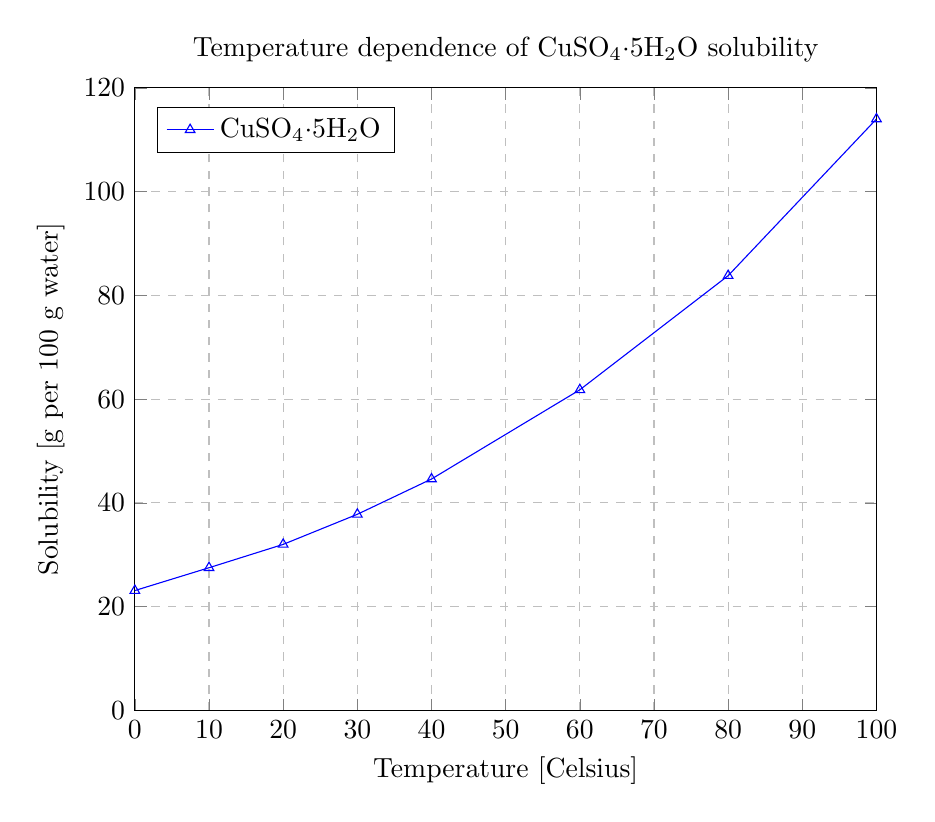
\begin{tikzpicture}
\begin{axis}[
    title={Temperature dependence of CuSO$_4\cdot$5H$_2$O solubility},
    xlabel={Temperature [Celsius]},
    ylabel={Solubility [g per 100 g water]},
    xmin=0, xmax=100,
    ymin=0, ymax=120,
    legend pos=north west,
    xmajorgrids=true,
    ymajorgrids=true,
    grid style=dashed,
]

\addplot[
    color=blue,
    mark=triangle,
    ]
    coordinates {
    (0,23.1)(10,27.5)(20,32)(30,37.8)(40,44.6)(60,61.8)(80,83.8)(100,114)
    };
    \legend{CuSO$_4\cdot$5H$_2$O}
    
\end{axis}
\end{tikzpicture}

\end{document}